% Chapter 3

\chapter{A Representation Learning Framework for Gene Regulatory Network Inference from Time-series Expression Data} % Main chapter title

\label{Chapter3} % For referencing the chapter elsewhere, use \ref{Chapter1} 

%----------------------------------------------------------------------------------------

% Define some commands to keep the formatting separated from the content 
% \newcommand{\keyword}[1]{\textbf{#1}}
% \newcommand{\tabhead}[1]{\textbf{#1}}
% \newcommand{\code}[1]{\texttt{#1}}
% \newcommand{\file}[1]{\texttt{\bfseries#1}}
% \newcommand{\option}[1]{\texttt{\itshape#1}}

%----------------------------------------------------------------------------------------

\section{Abstract}
GRNs describe the complex regulatory relationships that govern gene expression and play a central role in fundamental biological processes such as development, cellular differentiation, and responses to environmental perturbations. Inferring GRNs from time-series gene expression data is therefore a key problem in computational biology. However, this task remains challenging due to the high dimensionality of expression profiles, limited sample sizes, intrinsic noise, and the dynamic and nonlinear nature of gene regulation. Classical GRN inference methods typically rely on explicit statistical or mechanistic models, such as correlation analysis, regression frameworks, mutual information estimation, or Bayesian formulations. While these approaches have provided important insights, they often depend on strong assumptions regarding linearity, time delays, or the number of candidate regulators, which can limit robustness and generalizability across datasets.

In this thesis, we propose a novel data representation framework that reformulates GRN inference as a binary classification problem over gene pairs. Instead of explicitly modeling regulatory dynamics through predefined equations or probabilistic structures, the proposed framework encodes each potential regulatory interaction into a fixed-dimensional feature vector that jointly captures temporal expression dynamics and local structural context. This representation enables the direct application of a wide range of supervised machine learning models, allowing regulatory relationships to be inferred in a data-driven and assumption-free manner. By avoiding heuristic parameters such as fixed time lags or predefined regulator sets, the framework improves flexibility and reduces sensitivity to dataset-specific tuning.

A key property of the proposed representation is its independence from the global size of the underlying network. Because regulatory interactions are encoded locally, interactions drawn from networks of different sizes share a consistent representation. This scale invariance facilitates cross-network generalization and enables training data to be constructed from mixtures of networks with varying sizes, which is particularly beneficial for mitigating class imbalance between interacting and non-interacting gene pairs. Moreover, once trained, the resulting classifiers support efficient inference, as models can be trained once and reused to predict regulatory interactions across large collections of networks.

We evaluate the proposed approach on benchmark synthetic datasets generated from the \textit{Escherichia coli (E.coli)} regulatory network topology, considering both discrete-valued toy datasets and continuous-valued time series data, and across multiple network sizes. Experimental results demonstrate that the proposed framework achieves consistently strong performance across different data generation regimes and network scales, outperforming traditional GRN inference approaches that rely on explicit statistical or model-based assumptions. These findings highlight the robustness, scalability, and practical applicability of the proposed representation learning framework.

Overall, this work demonstrates that reframing GRN inference through a principled data representation and supervised learning paradigm provides a flexible and scalable alternative to traditional modeling-driven approaches. The proposed framework offers a general foundation for integrating modern machine learning techniques into GRN reconstruction and holds promise for future applications in systems biology and large scale genomic data analysis.

\section{Introduction}
GRNs describe the complex and coordinated interactions among genes and their regulatory elements, which collectively govern essential biological processes such as cell differentiation, development, and cellular responses to environmental stimuli. Accurate inference of GRNs from time-series gene expression data is therefore a fundamental problem in computational biology, as it provides mechanistic insights into gene regulation and supports downstream applications in disease modeling, precision medicine, synthetic biology, and drug discovery. However, reconstructing GRNs from expression data remains challenging due to the high dimensionality of genomic measurements, the presence of stochastic noise, and the limited number of temporal samples typically available in experimental settings.

A wide range of computational approaches has been proposed for GRN inference, spanning from classical statistical techniques to more advanced machine learning models. Early correlation based methods, such as Pearson and Spearman correlation, infer regulatory relationships by measuring pairwise linear or monotonic associations between gene expression profiles \parencite{langfelder2008, guo2014inferring}. Although computationally efficient, these approaches fail to capture complex nonlinear dependencies and are highly sensitive to noise, which often results in inflated false positive rates. Regression based methods, including GENIE3 \parencite{huynhthu2010}, fused LASSO models \parencite{omranian2016gene}, and KFLR \parencite{pirgazi2018robust}, extend this paradigm by modeling gene expression as a function of potential regulators while imposing sparsity constraints to reduce spurious interactions. Despite improved specificity, these methods rely on explicit functional assumptions, such as linearity or tree-based relationships, and typically require large sample sizes to achieve stable and reliable inference.

Mutual information based approaches, such as ARACNE \parencite{margolin2006}, CLR \parencite{faith2007}, and MIDNI \parencite{anh2023mutual}, relax linearity assumptions by quantifying general statistical dependencies between gene pairs. While these methods are more effective at detecting nonlinear interactions and exhibit improved robustness to noise, they often depend on discretization of continuous expression values, which can lead to information loss, and they face difficulties in distinguishing direct regulatory effects from indirect associations. Probabilistic frameworks, including Bayesian networks \parencite{wilczynski2009} and dynamic Bayesian networks \parencite{ajmal2021dynamic, suter2022discovering}, further incorporate temporal dependencies and uncertainty modeling. Although theoretically well grounded, these approaches are computationally demanding and sensitive to prior assumptions, which limits their scalability to large networks and long time-series datasets.

More recently, task transformation or problem reformulation, has emerged as a promising strategy for addressing the complexity of GRN inference. Instead of explicitly modeling regulatory functions or dependency structures, several methods recast GRN reconstruction into supervised learning tasks that are more amenable to modern machine learning algorithms. For example, CNNGRN \parencite{Gao2023} reformulates GRN inference as a binary classification problem by constructing joint representations of gene expression profiles and network features, enabling convolutional neural networks to capture spatial and temporal patterns. Similarly, MKL-GRNI \parencite{Wani2021} adopts a supervised classification framework at the transcription factor level and integrates multi-omics data through multiple kernel learning to improve robustness against noise and high dimensionality. GRNBoost2 \parencite{Moerman2019} reframes GRN inference as a regression based ranking task, which is subsequently converted into a binary classification problem to identify high confidence regulatory interactions, leveraging gradient boosting to scale to large single cell datasets.

Despite their demonstrated effectiveness, these task transformation based approaches share several common limitations that restrict their general applicability. In particular, they often rely on complex or method specific data representations that are difficult to interpret biologically and may not generalize well across different network sizes or experimental conditions. Moreover, temporal expression dynamics and regulatory structural context are typically encoded separately or indirectly, which limits the ability of the models to jointly capture complementary aspects of gene regulation. In addition, many existing formulations depend on predefined assumptions, such as fixed time delays, selected candidate regulators, or kernel configurations, which can constrain flexibility and hinder robustness when applied to heterogeneous datasets.

Motivated by these shared limitations, we propose a novel data representation framework that reformulates GRN inference as a binary classification problem through a unified and compact encoding of gene pair relationships. By jointly representing time-series expression dynamics and regulatory structural information within a standardized vector space, the proposed framework eliminates the need for explicit assumptions regarding time lags or regulator selection, thereby enabling assumption-free inference. This representation facilitates the direct application of a broad class of supervised learning models that have been extensively validated in other high-dimensional domains, allowing the proposed approach to leverage their robustness, scalability, and predictive power. Furthermore, the standardized nature of the representation enables seamless integration of data across networks of varying sizes, which supports cross-network learning and alleviates class imbalance, a persistent challenge in supervised GRN inference.

Empirical evaluations on benchmark GRN datasets demonstrate that the proposed method consistently outperforms existing approaches in terms of predictive accuracy and computational efficiency. These results highlight the potential of the proposed task transformation framework to overcome key limitations of both traditional and recent machine learning based GRN inference methods, providing a scalable, flexible, and biologically meaningful solution for reconstructing gene regulatory networks from time-series expression data.
\section{Materials and methods}
\subsection{Related works}
To evaluate the proposed method, which reformulates GRN inference as a binary classification task, we compare it with representative approaches spanning major paradigms for time-series GRN inference, including tree based, regression based, mutual information based, and Bayesian model based methods. Tree based methods are represented by JUMP3 \parencite{HuynhThu2015}, which combines decision trees with dynamic programming to infer regulatory interactions from time-series data. Regression based approaches are represented by Inferelator \parencite{greenfield2010dream4} and TSNI \parencite{bansal2006inference}, which model gene expression dynamics using linear regression or linear differential equation frameworks with time-lagged predictors. Mutual information based methods are represented by CLR-lag \parencite{faith2007}, which extends the CLR framework by incorporating temporal delays to capture dynamic regulatory relationships. Bayesian model based approaches are represented by G1DBN \parencite{Lebre2007}, a Dynamic Bayesian Network method that explicitly models temporal conditional dependencies in gene regulation from time-series data.

\subsection{Performance Metrics}\label{metrics}
In this study, we employ the Precision-Recall (PR) curve and its corresponding Area Under the Precision-Recall Curve (AUPR) as the primary evaluation metrics to assess the performance of gene network inference. The PR curve plots the trade-off between precision (the proportion of true positive predictions among all positive predictions) and recall (the proportion of true positives detected among all actual positives) across various classification thresholds. Unlike the ROC curve, which may present an overly optimistic view in imbalanced datasets, the PR curve is more informative in scenarios where the positive class (true gene-gene interactions) is significantly outnumbered by the negative class (non-interacting pairs), as commonly seen in biological networks. The AUPR summarizes the PR curve into a single scalar value between 0 and 1, where a value of 1 indicates perfect classification and a value close to 0 suggests random or poor predictive performance. Therefore, AUPR serves as a robust indicator of model effectiveness in the context of sparse and noisy biological data.
\section{Our proposed model}

\subsection{Data representation}\label{transformation}
Inferring gene regulatory networks from time series expression data remains challenging due to the complex interplay between temporal dynamics and network structure, as well as the severe class imbalance between interacting and non-interacting gene pairs. Traditional approaches often rely on handcrafted assumptions, such as fixed time delays or predefined regulator sets, which can limit their generalizability across datasets and network scales. To address these limitations, we seek a representation that directly encodes dynamic expression information at the level of individual gene pairs, while remaining agnostic to network size and structural priors. Such a representation should enable the application of supervised learning techniques by transforming GRN inference into a standard classification problem, thereby leveraging advances in machine learning for scalable and robust network reconstruction. Motivated by these considerations, we introduce a novel representation of time series gene expression data that supports supervised learning–based GRN inference. Instead of representing gene interactions using gene identifiers, we encode each pairwise interaction by concatenating their corresponding gene expression vectors over time.

Given a time series data set with $T$ observed time points, the expression profile of a gene $G_i$ is denoted by a vector:

$$
\mathbf{V}_i = \{v_{i}^{(1)}, v_{i}^{(2)}, \ldots, v_{i}^{(T)}\}
$$

where $v_{i}^{(t)}$ represents the expression value of gene $G_i$ at time point $t$.

Each regulatory interaction in the gold standard file is given in the form of a directed edge $G_j \rightarrow G_i$, labeled 1 if an interaction exists and 0 otherwise. For each such gene pair, we construct a feature vector by concatenating the expression vectors of the regulator and the target:

$$
\mathbf{x}_{(j,i)} = \mathbf{V}_j \oplus \mathbf{V}_i \in \mathbb{R}^{2T}
$$

with the corresponding binary label:

$$
y_{(j,i)} = 
\begin{cases}
1, & \text{if } G_j \rightarrow G_i \text{ exists} \\
0, & \text{otherwise}
\end{cases}
$$

By applying this transformation across all gene pairs in the gold standard, we obtain a labeled dataset $\mathcal{D} = \{ (\mathbf{x}_{(j,i)}, y_{(j,i)}) \}$, where each sample represents a regulatory interaction.

This representation framework confers several notable advantages for GRN inference. First, by integrating both the structural context of regulatory interactions and the temporal dynamics of gene expression, it yields a more informative feature space that captures complementary aspects of regulatory behavior. This joint encoding enhances the model’s capacity to detect true interactions, outperforming approaches that rely solely on temporal expression profiles. Second, the method operates in an assumption-free manner, obviating the need for predefined parameters, such as time delays or the number of candidate regulators, requirements that often constrain traditional inference techniques. Specifically, temporal dependencies are implicitly captured through the encoded expression dynamics rather than being imposed via fixed time-lag assumptions, while regulatory candidates are learned directly from data without restricting the search space to a predefined subset. Third, the reformulation of the GRN reconstruction problem as a binary classification task enables the direct application of a broad class of supervised learning models, facilitating robust and scalable prediction. Finally, the standardized vector representation allows for seamless integration of data across networks of varying sizes, thereby supporting cross network generalization and mitigating class imbalance which is an inherent difficulty in supervised GRN inference tasks. In large networks (e.g., size 100), true regulatory interactions typically constitute only a small fraction of all possible gene pairs, leading to severe imbalance between interaction and non-interaction classes. Under this unified representation, interaction samples derived from networks of smaller sizes (e.g., size 10 or size 50) can be naturally incorporated into the training set to enrich positive examples. This strategy is feasible because all gene pairs are encoded into fixed-length feature vectors with identical dimensionality, regardless of network size, enabling effective knowledge transfer across datasets and improving model robustness in large scale settings.

\subsection{The model}
The Figure ~\ref{chapter3_framework} presents the entire framework of our proposed approach. It begins with a collection of gold standard gene regulatory network structures that specify the true regulatory interactions between gene pairs. These networks provide the structural foundation from which simulated expression dynamics are produced. Time-series expression profiles for every network structure are generated using the GeneNetWeaver (GNW) simulator. Each profile contains the expression trajectories of all genes across \(T\) time steps. These expression profile is then converted into a supervised learning dataset using the representation procedure described in ~\ref{transformation}. This procedure transforms raw temporal expression values into feature and label pairs that encode the local regulatory context of each candidate interaction. The resulting represented dataset forms a unified feature space that is compatible with a wide variety of machine learning algorithms that include linear methods, tree based approaches, ensemble techniques, probabilistic models, non parametric classifiers, and neural architectures. In particular, we employ Linear Regression (LR), Decision Tree (DT), Random Forest (RF), Light Gradient Boosting Machine (LightGBM), Extreme Gradient Boosting (XGBoost), Gaussian Naive Bayes (GNB), K Nearest Neighbors (KNN), and a Multi Layer Perceptron (MLP). (MLP).This comprehensive model set ensures that the evaluation reflects not only the effectiveness of the proposed data representation but also its general applicability across fundamentally different learning mechanisms. The parameter configurations applied to these models during the training process are detailed in Table ~\ref {chapter3_structure}. After training, all models are stored in a pool of classifier models, which allows users to select a preferred model when performing inference on new data. When presented with an unseen expression dataset, the inference pipeline assumes that the data contain exactly \(T\) observed time steps, matching the temporal length used during model training. Under this setting, the unseen expression profiles are directly transformed using the same representation strategy without requiring any additional preprocessing or temporal alignment. The number of observed time steps therefore constitutes the primary prerequisite for inference, and this parameter is typically well defined for most experimental time series datasets. Once the expression data are transformed into the represented feature space, a selected model from the classifier pool is applied to predict interaction labels for all candidate gene pairs. The final output of the inference pipeline is a binary label for each gene pair indicating interaction or non interaction. These pairwise labels are then assembled to reconstruct the inferred gene regulatory network.

\begin{figure*}[!t]
\centering
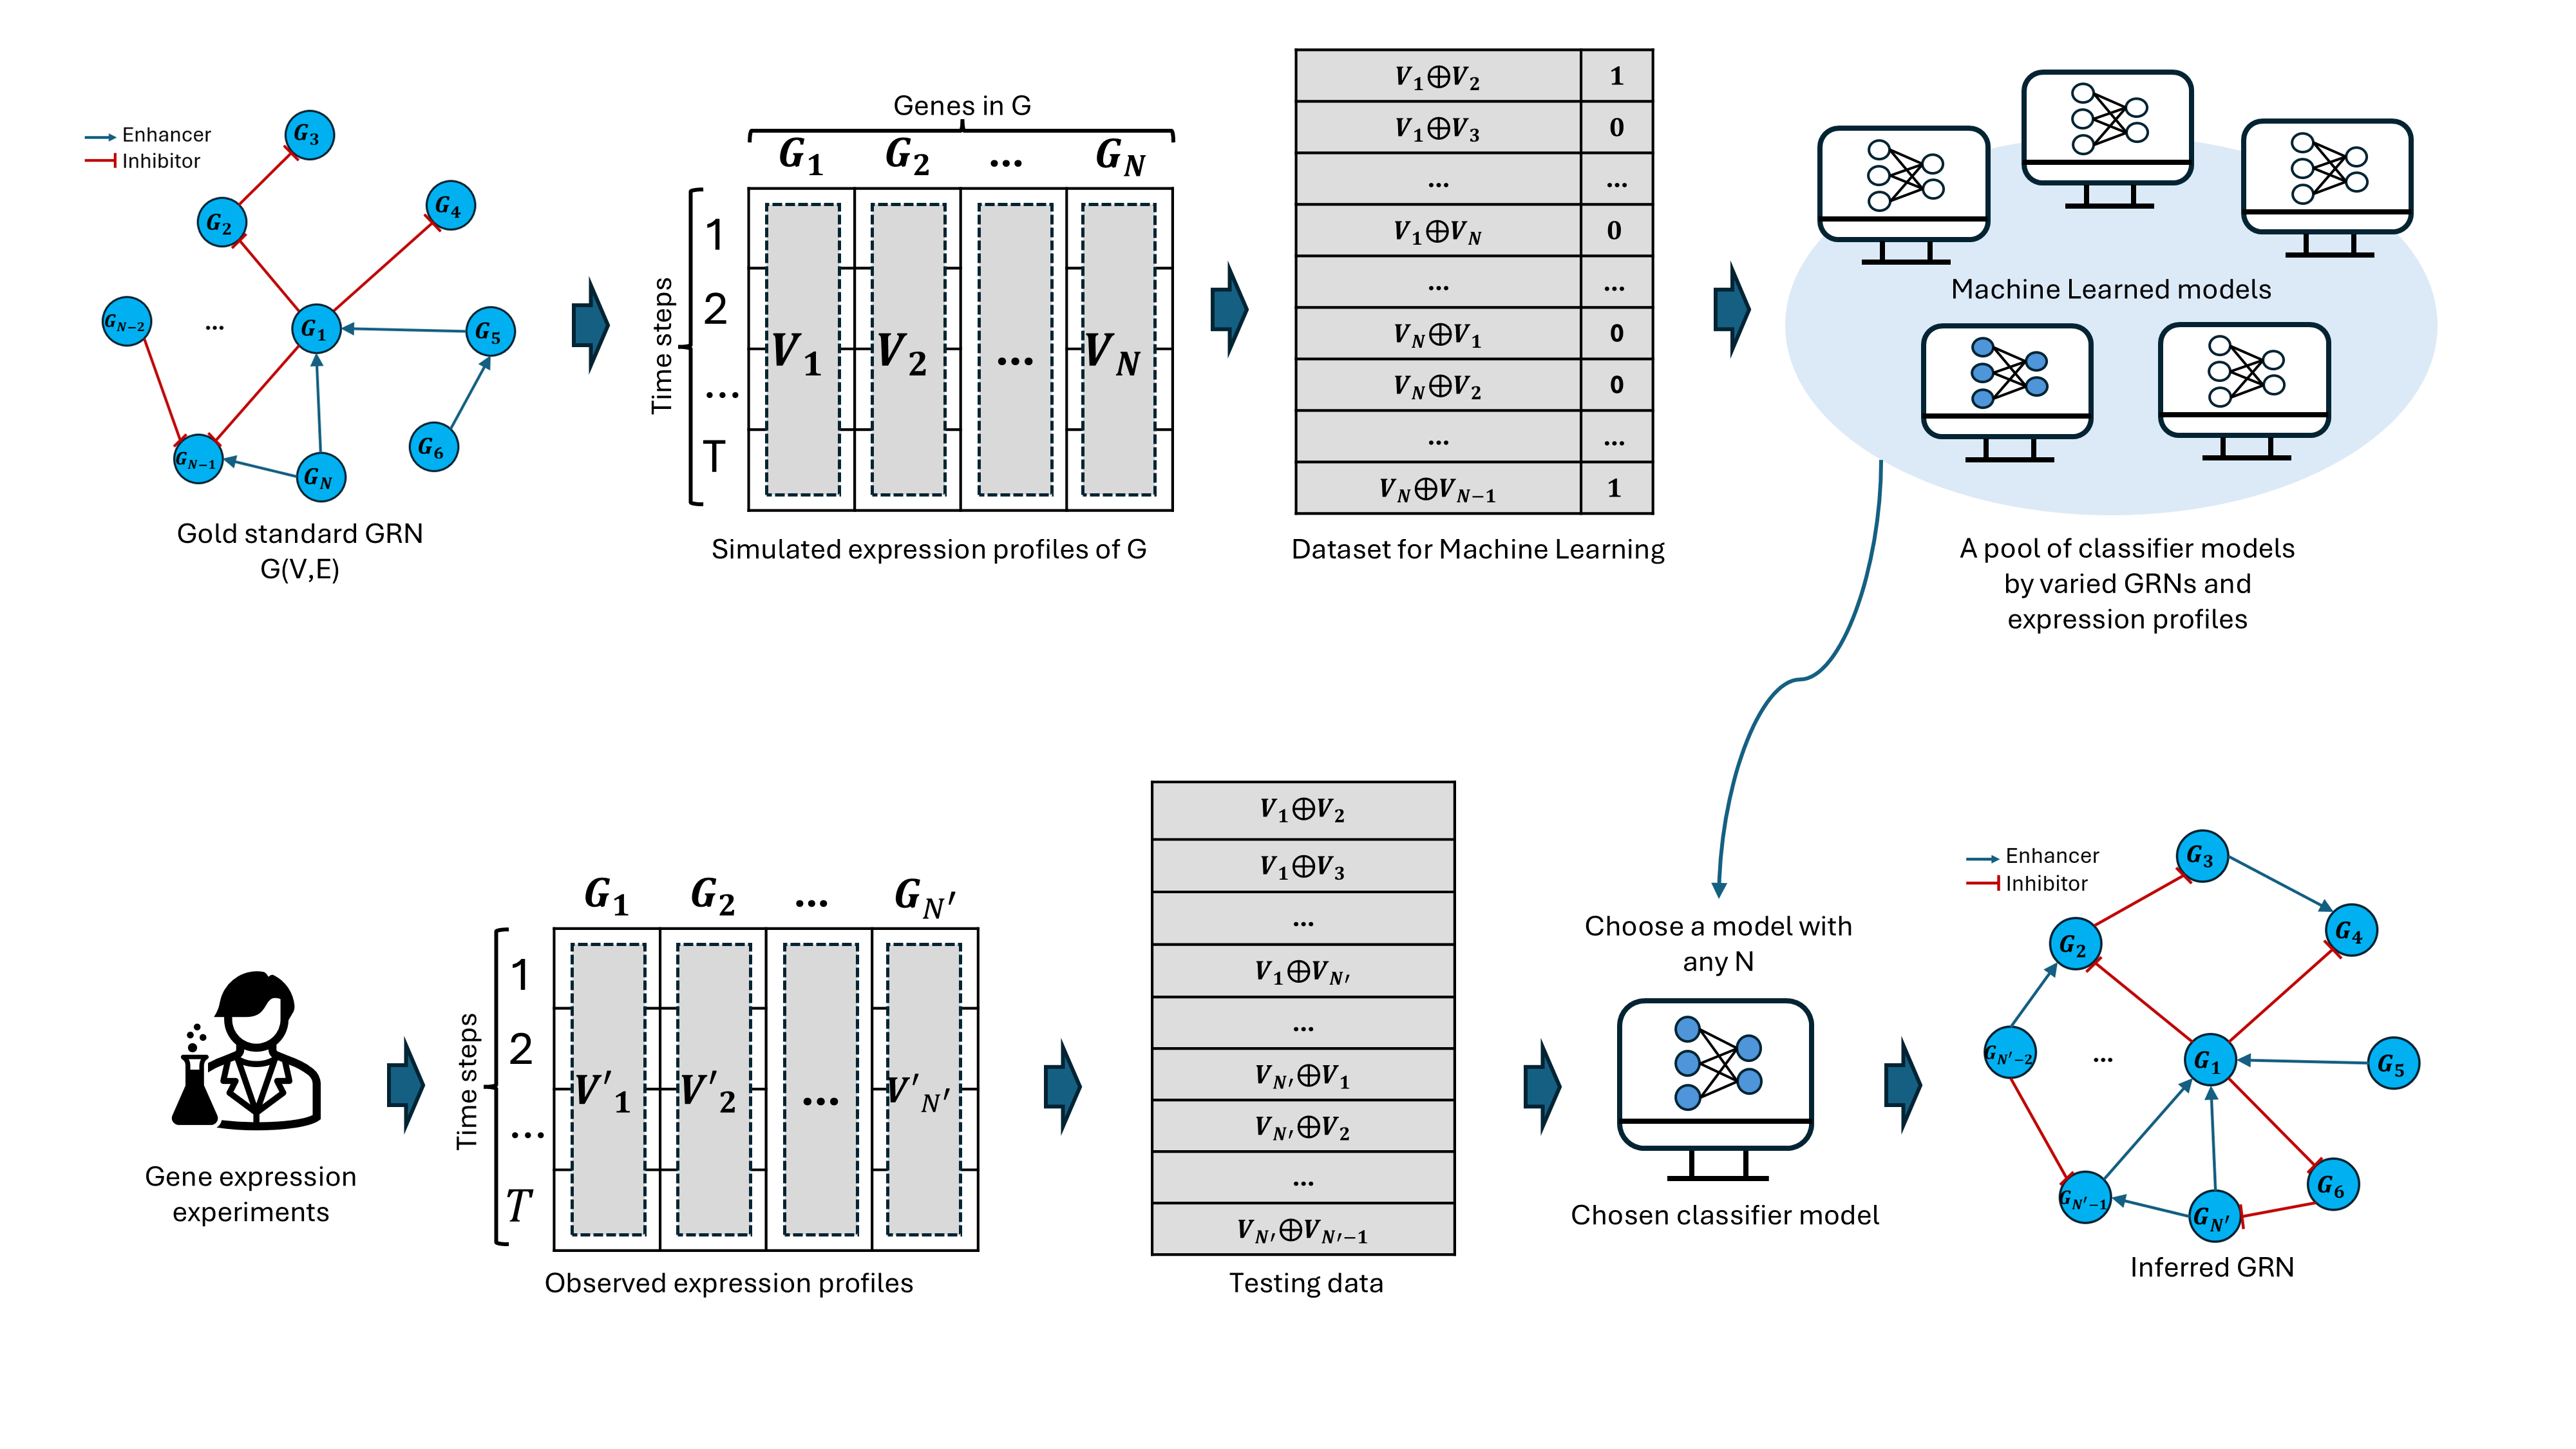
\includegraphics[width=1.05\linewidth]{Figures/chapter3_structure.png}
%{\color{black!20}\rule{438pt}{74pt}}
\caption{Overview of the proposed GRN inference framework. The key required input is the observed number of timesteps, which determines how simulated trajectories are aligned with the test instances. In contrast, network size is not a constraining factor, since the proposed representation enables models trained on networks of one size to generalize reliably to networks of different sizes. The framework produces pairwise interaction predictions for all gene pairs, which are then aggregated to reconstruct the inferred regulatory network.
}\label{chapter3_framework}
\end{figure*}


\begin{table}[!t]
\caption{The hyper parameters of classifiers\label{chapter3_structure}}%
\begin{tabular*}{\columnwidth}{@{\extracolsep\fill}llll@{\extracolsep\fill}}
\toprule
Model name & Parameter Name & Value \\
\midrule
% Linear Regression &\multirow{3}{*}{\multicolumn{1}{c}{Default setting}} &\\
Linear Regression &\multirow{3}{*}{Default setting} &\\
Gaussian Naive Bayes& &\\
Decision Tree& &\\
\cline{1-3}
\addlinespace[2pt]
\multirow{1}{*}{Random Forest } & Number of estimators &20\\
\multirow{1}{*}{KNN} & Number of neighbors &10\\
\addlinespace[2pt]
\cline{1-3}
\addlinespace[2pt]
\multirow{4}{*}{XGBoost} & Max-depth&3 \\
                        & Learning rate (eta)&0.1 \\
                        & Number of boosting rounds &100 \\
                        & Early stopping rounds &10 \\
\addlinespace[2pt]
\cline{1-3}
\addlinespace[2pt]
\multirow{5}{*}{LightGBM} & Boosting type&gbdt \\
                        & Leaves number&32 \\
                        & Learning rate &0.05 \\
                        & Feature fraction&0.9\\
                        & Number of boosting rounds &100 \\
\addlinespace[2pt]
\cline{1-3}
\addlinespace[2pt]
\multirow{6}{*}{MLP} & Number of hidden layers&5 \\
			&\shortstack{Activation functions \\in hidden layers}&relu \\
			&\shortstack{Activation function \\in the output layer}&sigmoid \\
			&Optimizer&Adam \\
                        & Learning rate&0.01 \\
                        & Loss function &mse \\
                        & Early stopping&yes\\
			& Patience&5\\
                        & Batch size &32 \\
                        & Epochs &100 \\
\botrule
\end{tabular*}
\end{table}
\section{Experimental Result}
\subsection{Performance on Toy datasets}
\textbf{Evaluation Across Machine Learning Models}: To assess the adaptability of the proposed representation on discretized data and networks with known structured topologies, we constructed synthetic datasets based on the Barabási–Albert (BA) model, which generates scale-free network structures commonly observed in gene regulatory systems (see Algorithm S2 in the Supplementary Materials). Specifically, 20,000 networks of size 10, and 2,000 networks each of sizes 50 and 100 were generated for training. For validation and testing, the datasets comprised 2,000 networks of size 10 and 400 networks each of sizes 50 and 100. For each ground-truth network, discretized gene expression profiles with three expression levels (0, 1, and 2) were simulated across 50 time points using a stochastic dynamical process. This synthetic setup allows controlled evaluation of the proposed method under well-defined topological and temporal conditions, in contrast to the inherent variability and noise present in real-world biological data.
Detailed statistics of the synthetic datasets are summarized in Table~\ref {chapter3_toy_dataset}.\par
Figure ~\ref{chapter3_toys} compares the AUPR performance of various methods across network sizes 10, 50, and 100, corresponding to 2,000, 400, and 400 test networks, respectively. For each model, we report the mean ± standard deviation of AUPR metric. The baseline random predictor yielded AUPR = 0.268 ± 0.034 (size 10), 0.048 ± 0.003 (size 50), and 0.023 ± 0.001 (size 100), evidencing the growing difficulty of the inference task as network size and hence the candidate edge space increases. Across models, three patterns are salient. First, ensemble/tree-based methods are highly competitive and robust: RF attains the best aggregate performance with AUPR = 0.602 ± 0.093 (size 10), 0.515 ± 0.053 (size 50), and 0.503 ± 0.058 (size 100). LightGBM also performs well at smaller scales (0.413 ± 0.079 at size 10) but degrades more with size. Second, deep learning (MLP) captures complex, non-linear dependencies effectively at small scale (0.566 ± 0.097 at size 10) but its performance declines for larger networks (0.329 ± 0.045 at size 50 and 0.288 ± 0.034 at size 100), consistent with higher sample requirements for stable generalization. Third, GNB exhibits notable robustness at larger scales, achieving AUPR = 0.398 ± 0.141 (size 10), 0.480 ± 0.138 (size 50), and 0.511 ± 0.001 (size 100), which places GNB among the top performers for size 50–100. Other methods (LR, XGBoost, KNN, DT) show variable, often inferior performance depending on scale. These results highlight that the proposed network representation is sufficiently general to support diverse learning paradigms including probabilistic, tree-based, boosting, and neural approaches for the task of structure inference. In addition, model suitability strongly depends on the degree of imbalance and network size, with RF and GNB demonstrating superior robustness under high imbalance, while MLP excels when the network is smaller and data density is higher.

\begin{table*}[!t]
\caption{Summary of the synthetic toy datasets used for GRN inference, including network sizes, number of networks, and interaction statistics \label{chapter3_toy_dataset}}%
\centering
\renewcommand{\arraystretch}{1.2} % tăng chiều cao dòng
\begin{tabular*}{\textwidth}{@{\extracolsep\fill} >{\raggedright\arraybackslash}m{2.0cm}  >{\raggedright\arraybackslash}m{4.5cm}  >{\raggedright\arraybackslash}m{2cm} >{\raggedright\arraybackslash}m{2cm} >{\raggedright\arraybackslash}m{2cm} @{\extracolsep\fill}}
\toprule
\textbf{Type} & \textbf{Parameter's name} & \multicolumn{3}{c@{}}{\textbf{Network size}} \\
\cline{3-5}
 & & 10 & 50 & 100 \\
\midrule
\multirow{5}{*}{Training Set} 
 & Network structure number & 20,000 & 2,000 & 2,000 \\
 & Time series number per structure & 1 & 1 & 1 \\
 & Time step in each network & 50 & 50 & 50 \\
 & Total interactions (millions) & 1.8 & 4.9 & 19.8 \\
 & Positive versus negative interactions & 0.3357 & 0.0484 & 0.0292 \\
\midrule
\multirow{5}{*}{Validation/Test Set} 
 & Network structure number & 2,000 & 400 & 400 \\
 & Time series number per structure & 1 & 1 & 1 \\
 & Time step in each network & 50 & 50 & 50 \\
 & Total interactions (millions) & 0.18 & 0.98 & 3.96 \\
 & Positive versus negative interactions & 0.3351/0.334 & 0.0483/0.0483 & 0.0234/0.0233 \\
\botrule
\end{tabular*}
\end{table*}

\subsection{Performance on Escherichia coli datasets}\label{performance_on_ecoli}
The \textit{E.coli} datasets used in this study were generated using the GNW simulator based on \textit{E. coli} transcriptional regulatory networks. Three network sizes were considered: 10, 50, and 100 genes. For the size-10 configuration, the dataset comprises 200, 20, and 10 network structures for the training, validation, and test sets, respectively. For the larger configurations (sizes 50 and 100), 20 network structures were used for training and 4 for both validation and testing. Each network structure includes 100 distinct time-series experiments, capturing diverse dynamic behaviors under different perturbations. For efficiency and consistency across models, only two representative time-series were selected from each test network during evaluation to ensure comparable computational costs. Detailed dataset configurations and interaction statistics are summarized in Table~\ref{chapter3_ecoli_dataset}.

Consistent with the results observed on the synthetic datasets, the proposed data representation also enables machine learning models to perform effectively on the \textit{E. coli} datasets, the detailed results are visually presented in Figure ~\ref{chapter3_gwns}. A complete breakdown of the quantitative results for this experimental setting is provided in Supplementary Section 2. Across all network sizes of 10, 50, and 100, the learning-based approaches achieved substantially higher AUPR scores compared with traditional network inference methods such as Jump3, Inferelator, CLR-lag, TSNI, and G1DBN. For instance, at size 10, the average AUPR across all machine learning models reached 0.518 ± 0.251, far exceeding the scores of Jump3 (0.174 ± 0.076) and Inferelator (0.169 ± 0.079). A similar trend was observed for larger networks: at size 50, the average AUPR was 0.164 ± 0.074 compared with 0.050 ± 0.006 for Jump3 and 0.040 ± 0.007 for Inferelator; and at size 100, the corresponding values were 0.111 ± 0.030 versus 0.031 ± 0.005 and 0.027 ± 0.005, respectively. Among the individual models, the GNB consistently achieved the highest and most stable performance across all network sizes 0.566 ± 0.171 (size 10), 0.355 ± 0.083 (size 50), and 0.324 ± 0.055 (size 100). This robustness can be attributed to GNB’s probabilistic formulation and its inductive bias of conditional independence, which makes it resilient to high class imbalance and data sparsity known as two persistent challenges in gene regulatory network inference. These results emphasize that the proposed representation enables machine learning models, particularly GNB, to effectively capture the underlying gene–gene dependencies, outperforming traditional inference frameworks and demonstrating scalability to biologically grounded datasets.\par

We also conducted a series of analyses to assess how the amount of training data and the use of small size networks influence the predictive capability of our learning framework. For this experiment, rather than training all models as in the previous toy dataset evaluation, we specifically selected the GNB model. This choice was motivated by two key reasons: First, GNB demonstrated more stable performance across all network sizes compared to other models, facilitating a clear and consistent comparison. Second, GNB is computationally efficient, allowing faster training and reduced resource usage. Three GNB models were independently trained on size-10 networks, using training sets of 5,000, 10,000, and 20,000 network structures, respectively and evaluated on test sets of sizes 10, 50, and 100. Detailed quantitative outcomes are summarized in Figure ~\ref{chapter3_gwns_accross}. The complete results for this experimental setting is reported in Supplementary Section 3.

Varying the number of training structures reveals a clear, though saturating, improvement as the training set size increases. With 5,000 structures, the model achieved AUPRs of 0.573, 0.349, and 0.322 on test sizes 10, 50, and 100. Expanding the training data to 10,000 structures resulted in only marginal changes (0.578, 0.352, 0.325), while the 20,000-structure configuration yielded stronger gains primarily for size-10 tests (0.674) and moderate benefits for larger networks (0.373 and 0.333) (see Figure ~\ref{chapter3_gwns_accross} \textbf{a}). Notably, training on the smallest dataset already provides competitive performance compared with the largest dataset, while requiring substantially less computational time, as illustrated in Figure ~\ref{chapter3_gwns_accross} \textbf{b} (2.58, 2.86. 3.21). These observations highlight that even limited training sets can suffice to produce near-optimal predictions, offering a favorable trade-off between accuracy and training efficiency.

Importantly, the experiment also highlights a central advantage of our representation: network size becomes far less restrictive, as models trained exclusively on size-10 networks can generalize effectively to larger networks. The size-10 model trained with 20,000 structures attained AUPRs of 0.373 (size 50) and 0.333 (size 100), closely matching models trained directly on size-50 and size-100 datasets (0.359 and 0.326, respectively). In certain cases, the small-network model even outperformed the matching-size baseline. This property is especially valuable when considering the substantial increase in training time: models trained on size-50 and size-100 datasets required 3.79 and 4.27 time units, respectively, which is markedly higher than the time needed for size-10 training. (see Figure ~\ref{chapter3_gwns_accross} \textbf{b}).

\begin{table*}[!t]
\caption{Summary of the \textit{E.coli} dataset used for GRN inference, including network sizes, number of networks, and interaction statistics } \label{chapter3_ecoli_dataset}
\centering
\renewcommand{\arraystretch}{1.2} % tăng chiều cao dòng
\begin{tabular*}{\textwidth}{@{\extracolsep\fill} >{\raggedright\arraybackslash}m{2.0cm}  >{\raggedright\arraybackslash}m{4.5cm}  >{\raggedright\arraybackslash}m{2cm} >{\raggedright\arraybackslash}m{2cm} >{\raggedright\arraybackslash}m{2cm} @{\extracolsep\fill}}
\toprule
\textbf{Type} & \textbf{Parameter's name} & \multicolumn{3}{c@{}}{\textbf{Network size}} \\
\cline{3-5}
 & & 10 & 50 & 100 \\
\midrule
\multirow{5}{*}{Training Set} 
 & Network structure number & 200 & 20 & 20 \\
 & Time series number per structure & 100 & 100 & 100 \\
 & Time step in each network & 50 & 50 & 50 \\
 & Total interactions (millions) & 1.8 & 4.9 & 19.8 \\
 & Positive versus negative interactions & 0.1 & 0.08 & 0.01 \\
\midrule
\multirow{5}{*}{Validation/Test Set} 
 & Network structure number & 20/10 & 4 & 4 \\
 & Time series number per structure & 100/2 & 100/2 & 100/2 \\
 & Time step in each network & 50 & 50 & 50 \\
 & Total interactions (millions) & 0.18/$1.8\times 10^{-3}$ & 0.98/0.0196 & 3.96/0.079 \\
 & Positive versus negative interactions & 0.18/0.156 & 0.041/0.044 & 0.025/0.023 \\
\botrule
\end{tabular*}
\end{table*}

\begin{figure}[!t]%
\centering
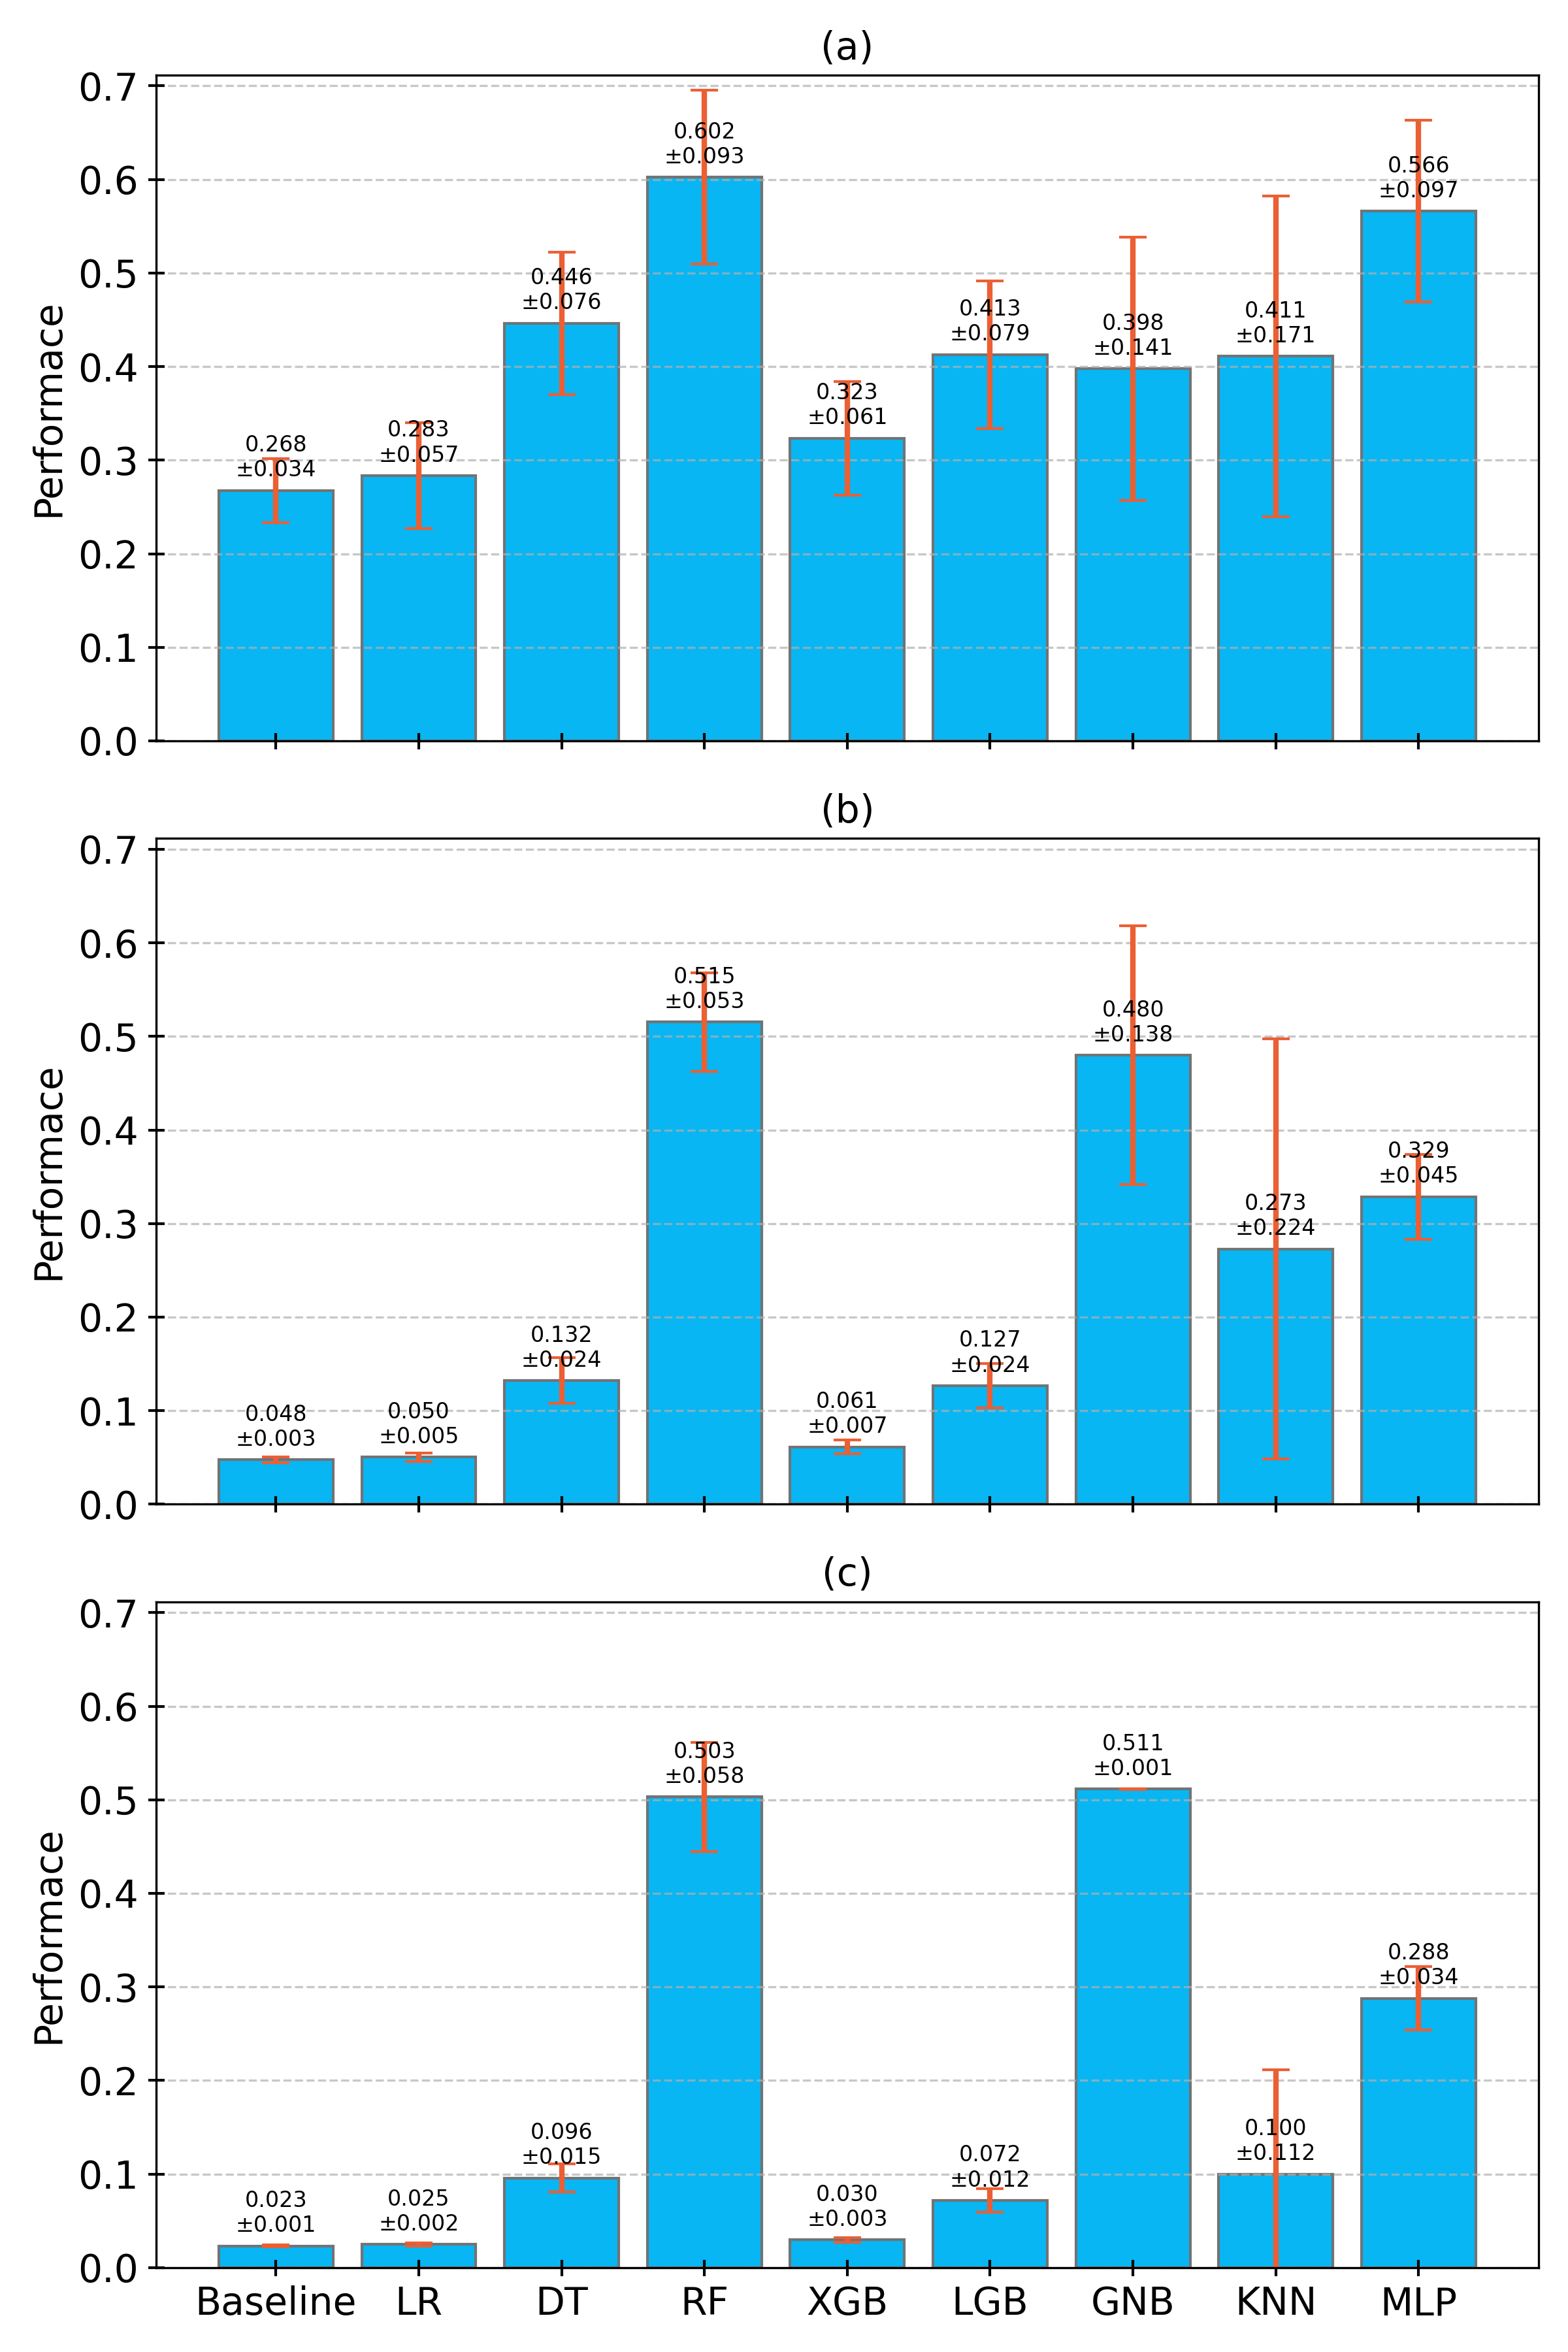
\includegraphics[width=1.0\linewidth]{Figures/chapter3_toys_single_size.png}
%{\color{black!20}\rule{438pt}{74pt}}
\caption{Figure shows the AUPR performance of different methods along the X-axis on the toy datasets. The Y-axis indicates the average AUPR values, with error bars representing the standard deviation. Subplots (\textbf{a}), (\textbf{b}), and (\textbf{c}) correspond to network sizes 10, 50, and 100, respectively, evaluated on 2,000, 400, and 400 test networks.}\label{chapter3_toys}
\end{figure}

\begin{figure}[!t]%
\centering
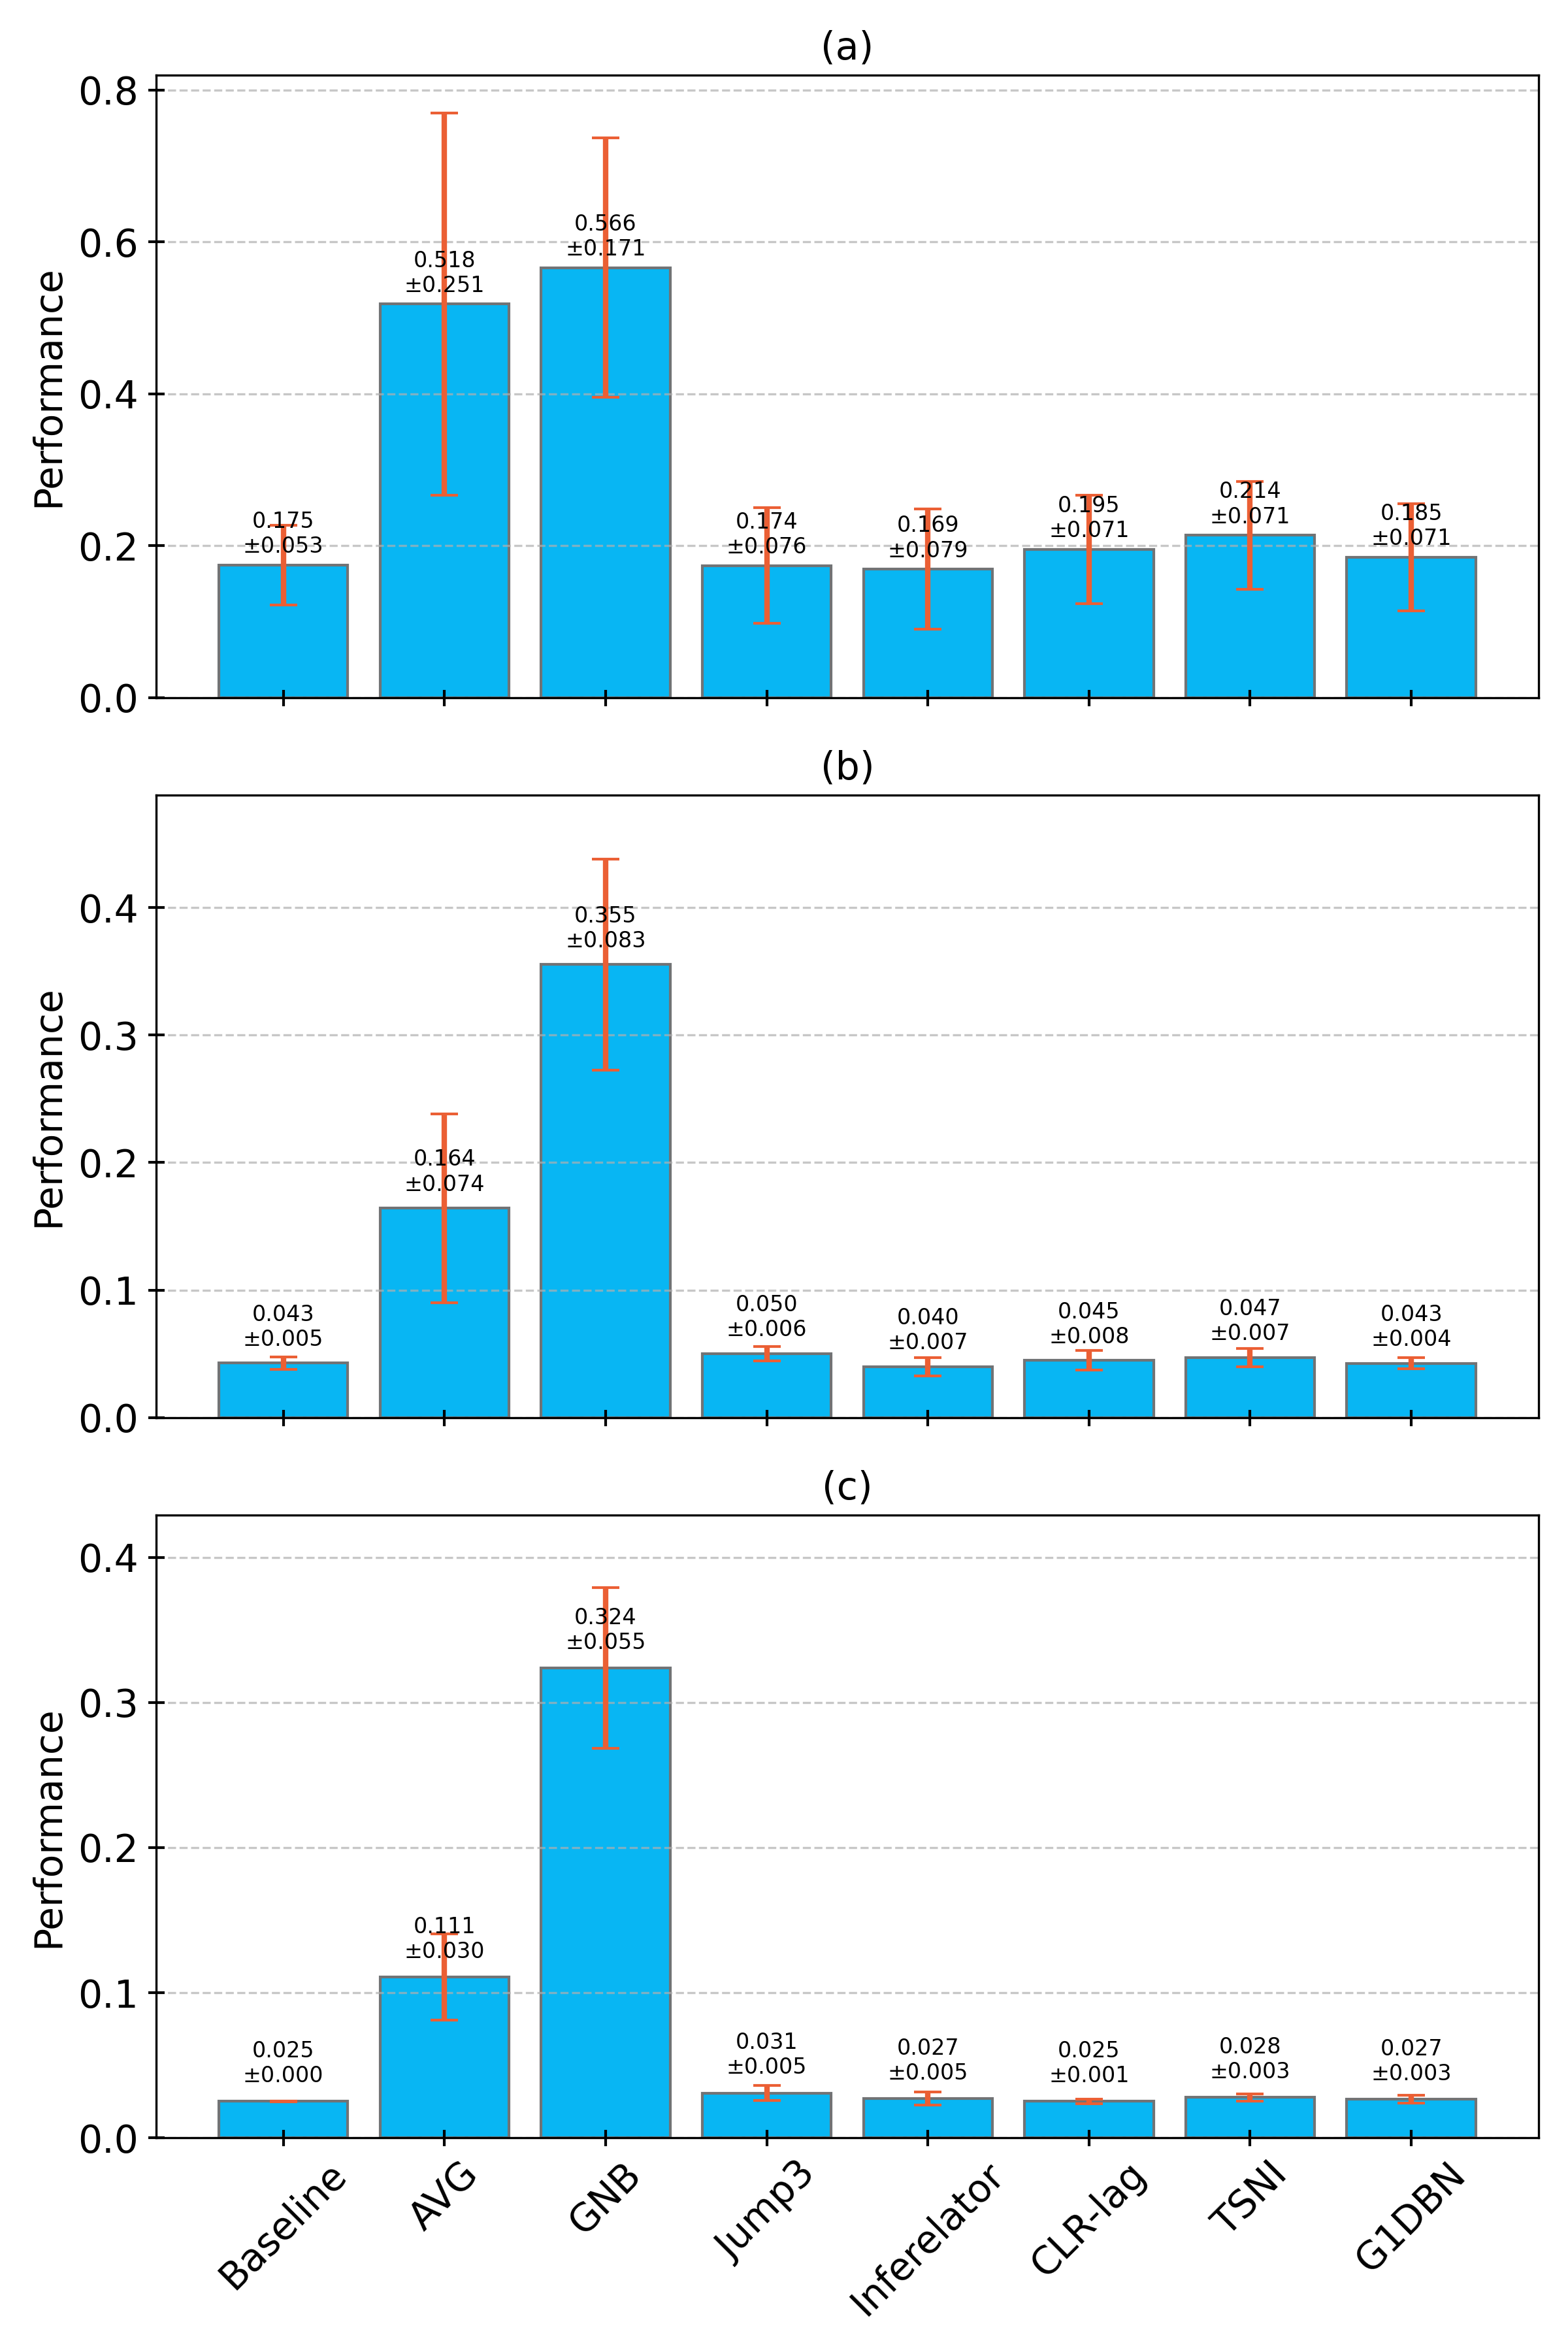
\includegraphics[width=1.0\linewidth]{Figures/chapter3_gwn_3.png}
%{\color{black!20}\rule{438pt}{74pt}}
\caption{Figure shows the AUPR performance of different methods along the X-axis on the \textit{E.coli} datasets. The Y-axis indicates the average AUPR values, with error bars representing the standard deviation. Subplots (\textbf{a}), (\textbf{b}), and (\textbf{c}) correspond to network sizes 10, 50, and 100, respectively, evaluated on 20, 8, and 8 test networks. }\label{chapter3_gwns}
\end{figure}



\begin{figure}[!t]%
\centering
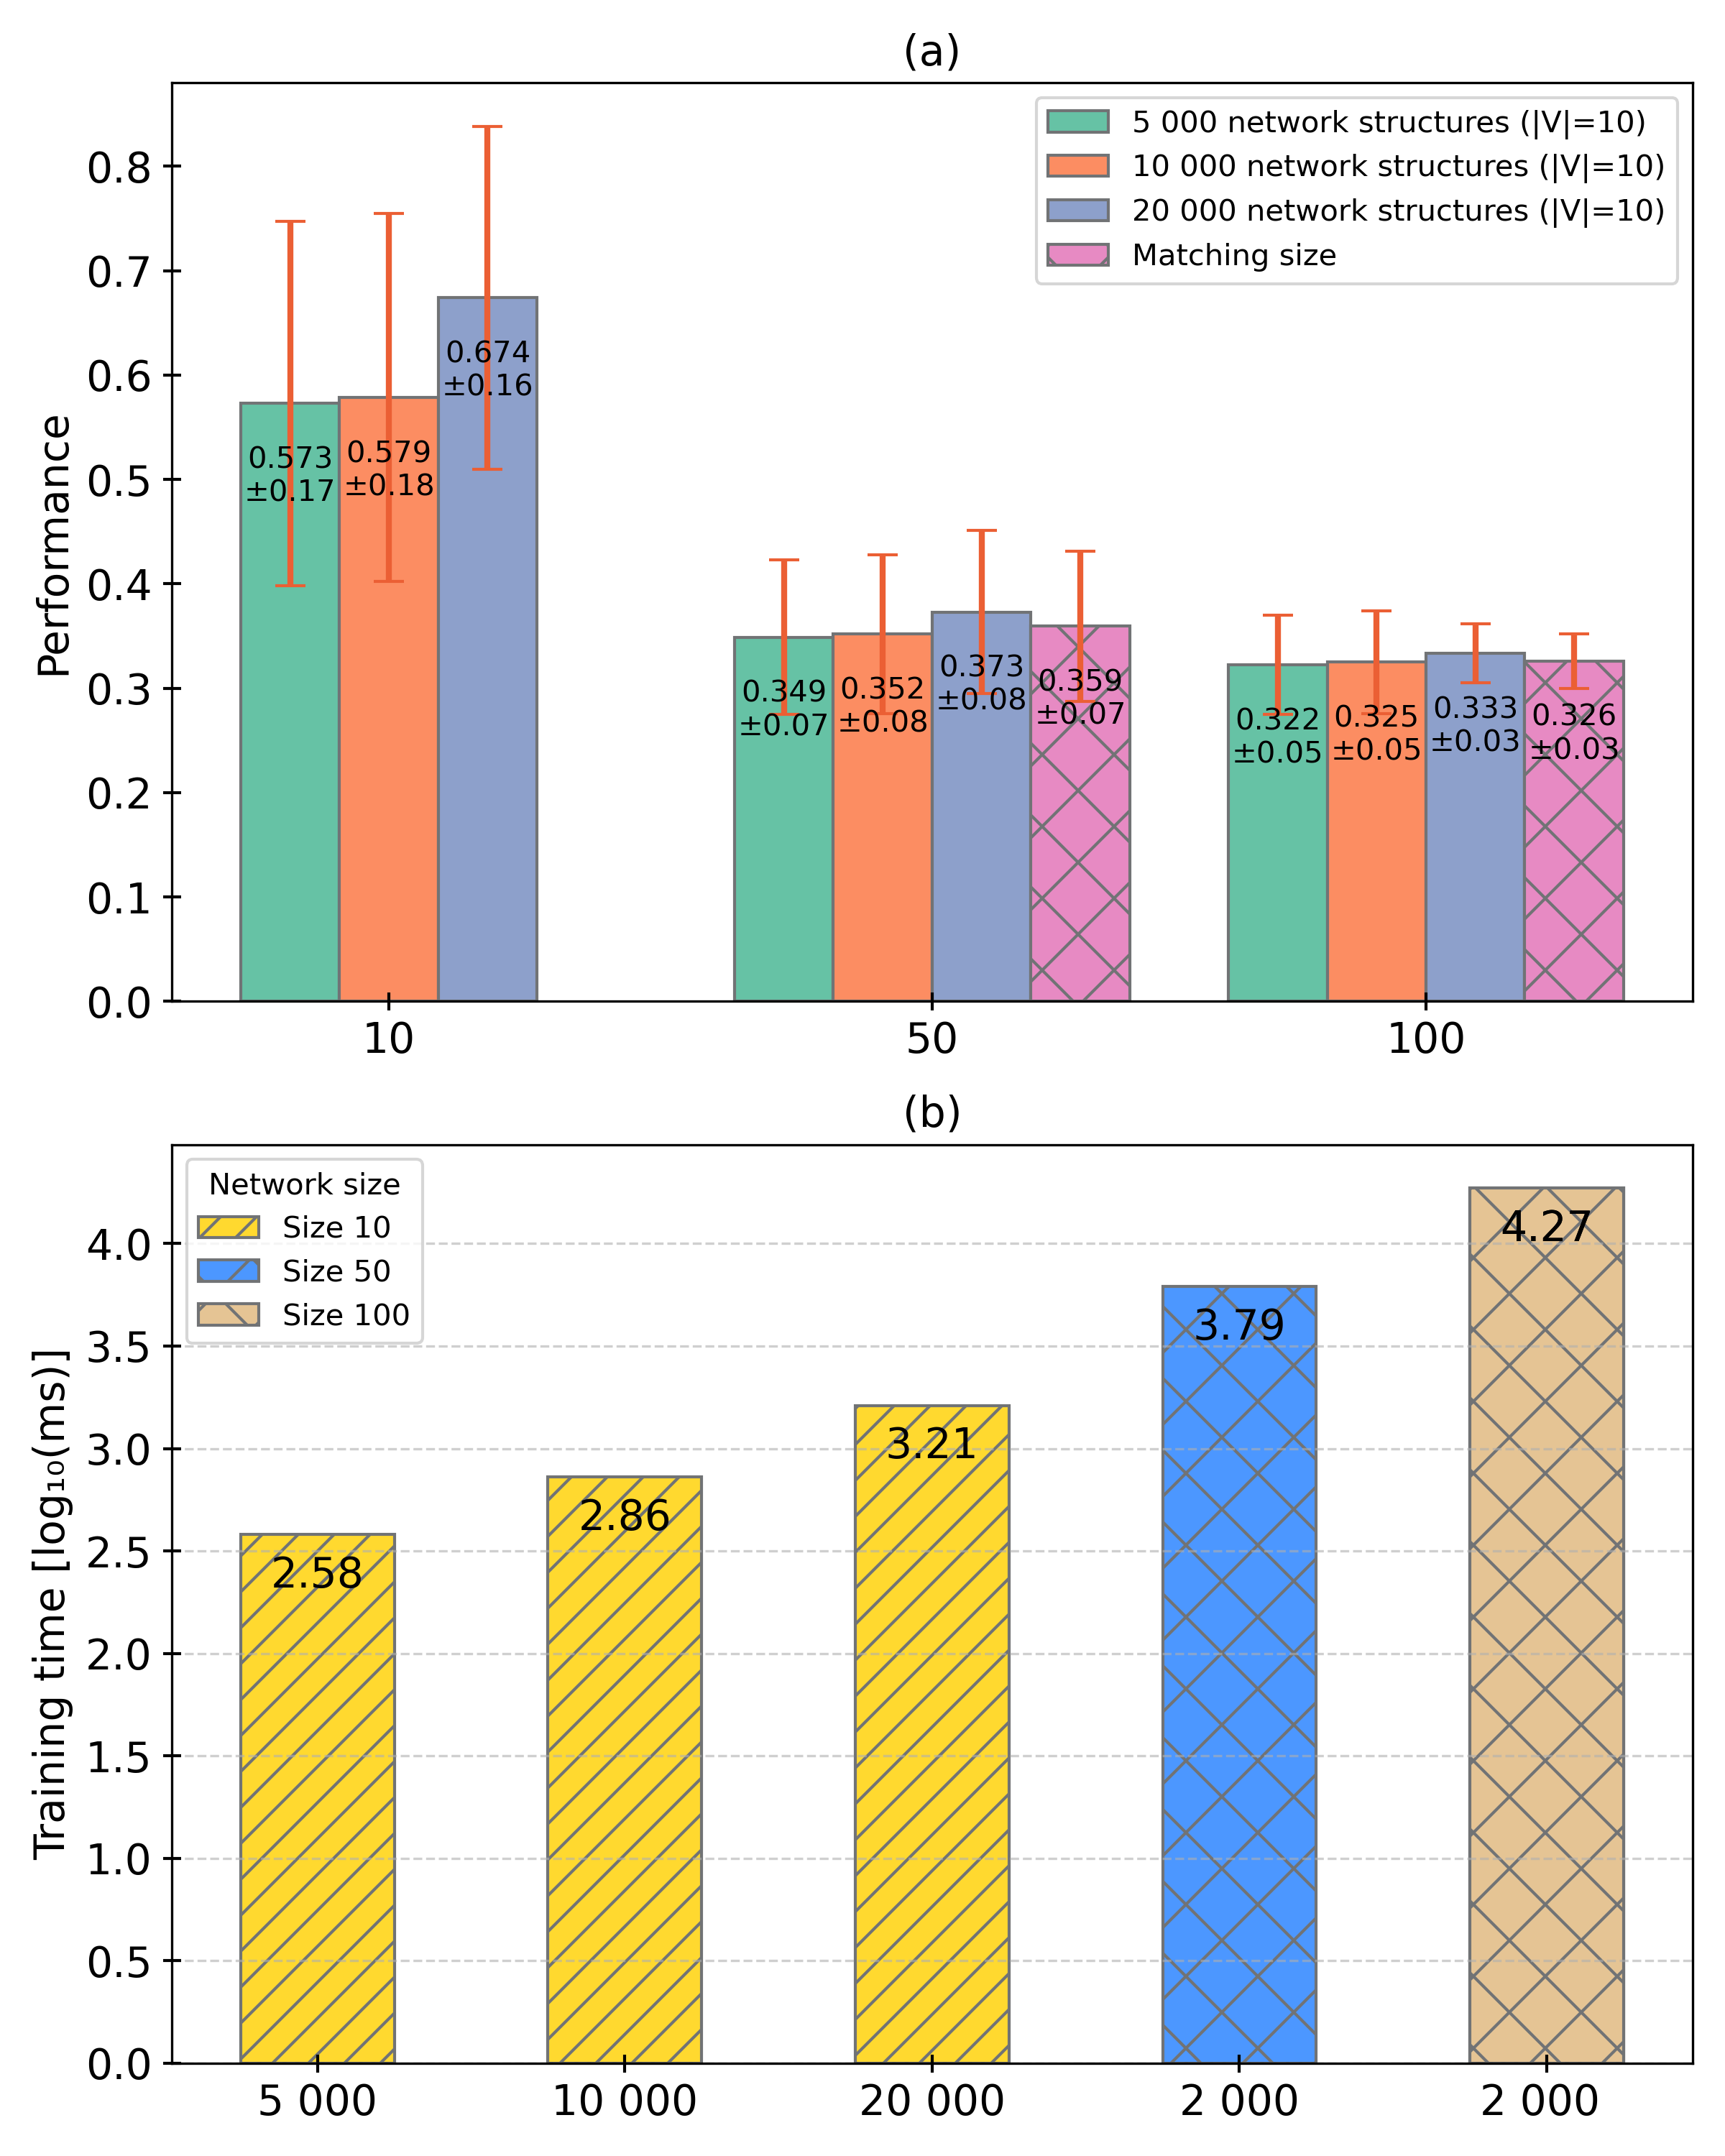
\includegraphics[width=1.0\linewidth]{Figures/chapter3_gwn_training_size.png}
%{\color{black!20}\rule{438pt}{74pt}}
\caption{Performance and training-time analysis across varying training-set sizes and network scales.
(\textbf{a}) Comparison of AUPR performance for three GNB models trained on datasets containing 5,000, 10,000, and 20,000 network structures (all with training network size of 10). Each model is evaluated on test networks of sizes 10, 50, and 100. Hatched bars denote the performance of models trained on matching network sizes (i.e., size-50 and size-100 training sets tested on size-50 and size-100 networks), included as baselines for comparison. The x-axis indicates the size of the testing network, and the y-axis reports AUPR. (\textbf{b}) Training-time comparison across datasets differing in both the number of network structures and the network size. The x-axis lists the training-set configurations (size-10 with 5 000, 10 000, and 20 000 structures, followed by size-50 and size-100 datasets, each has 2 000 network structures), and the y-axis reports the training time in log10-scaled milliseconds.}\label{chapter3_gwns_accross}
\end{figure}


\begin{figure}[!t]%
\centering
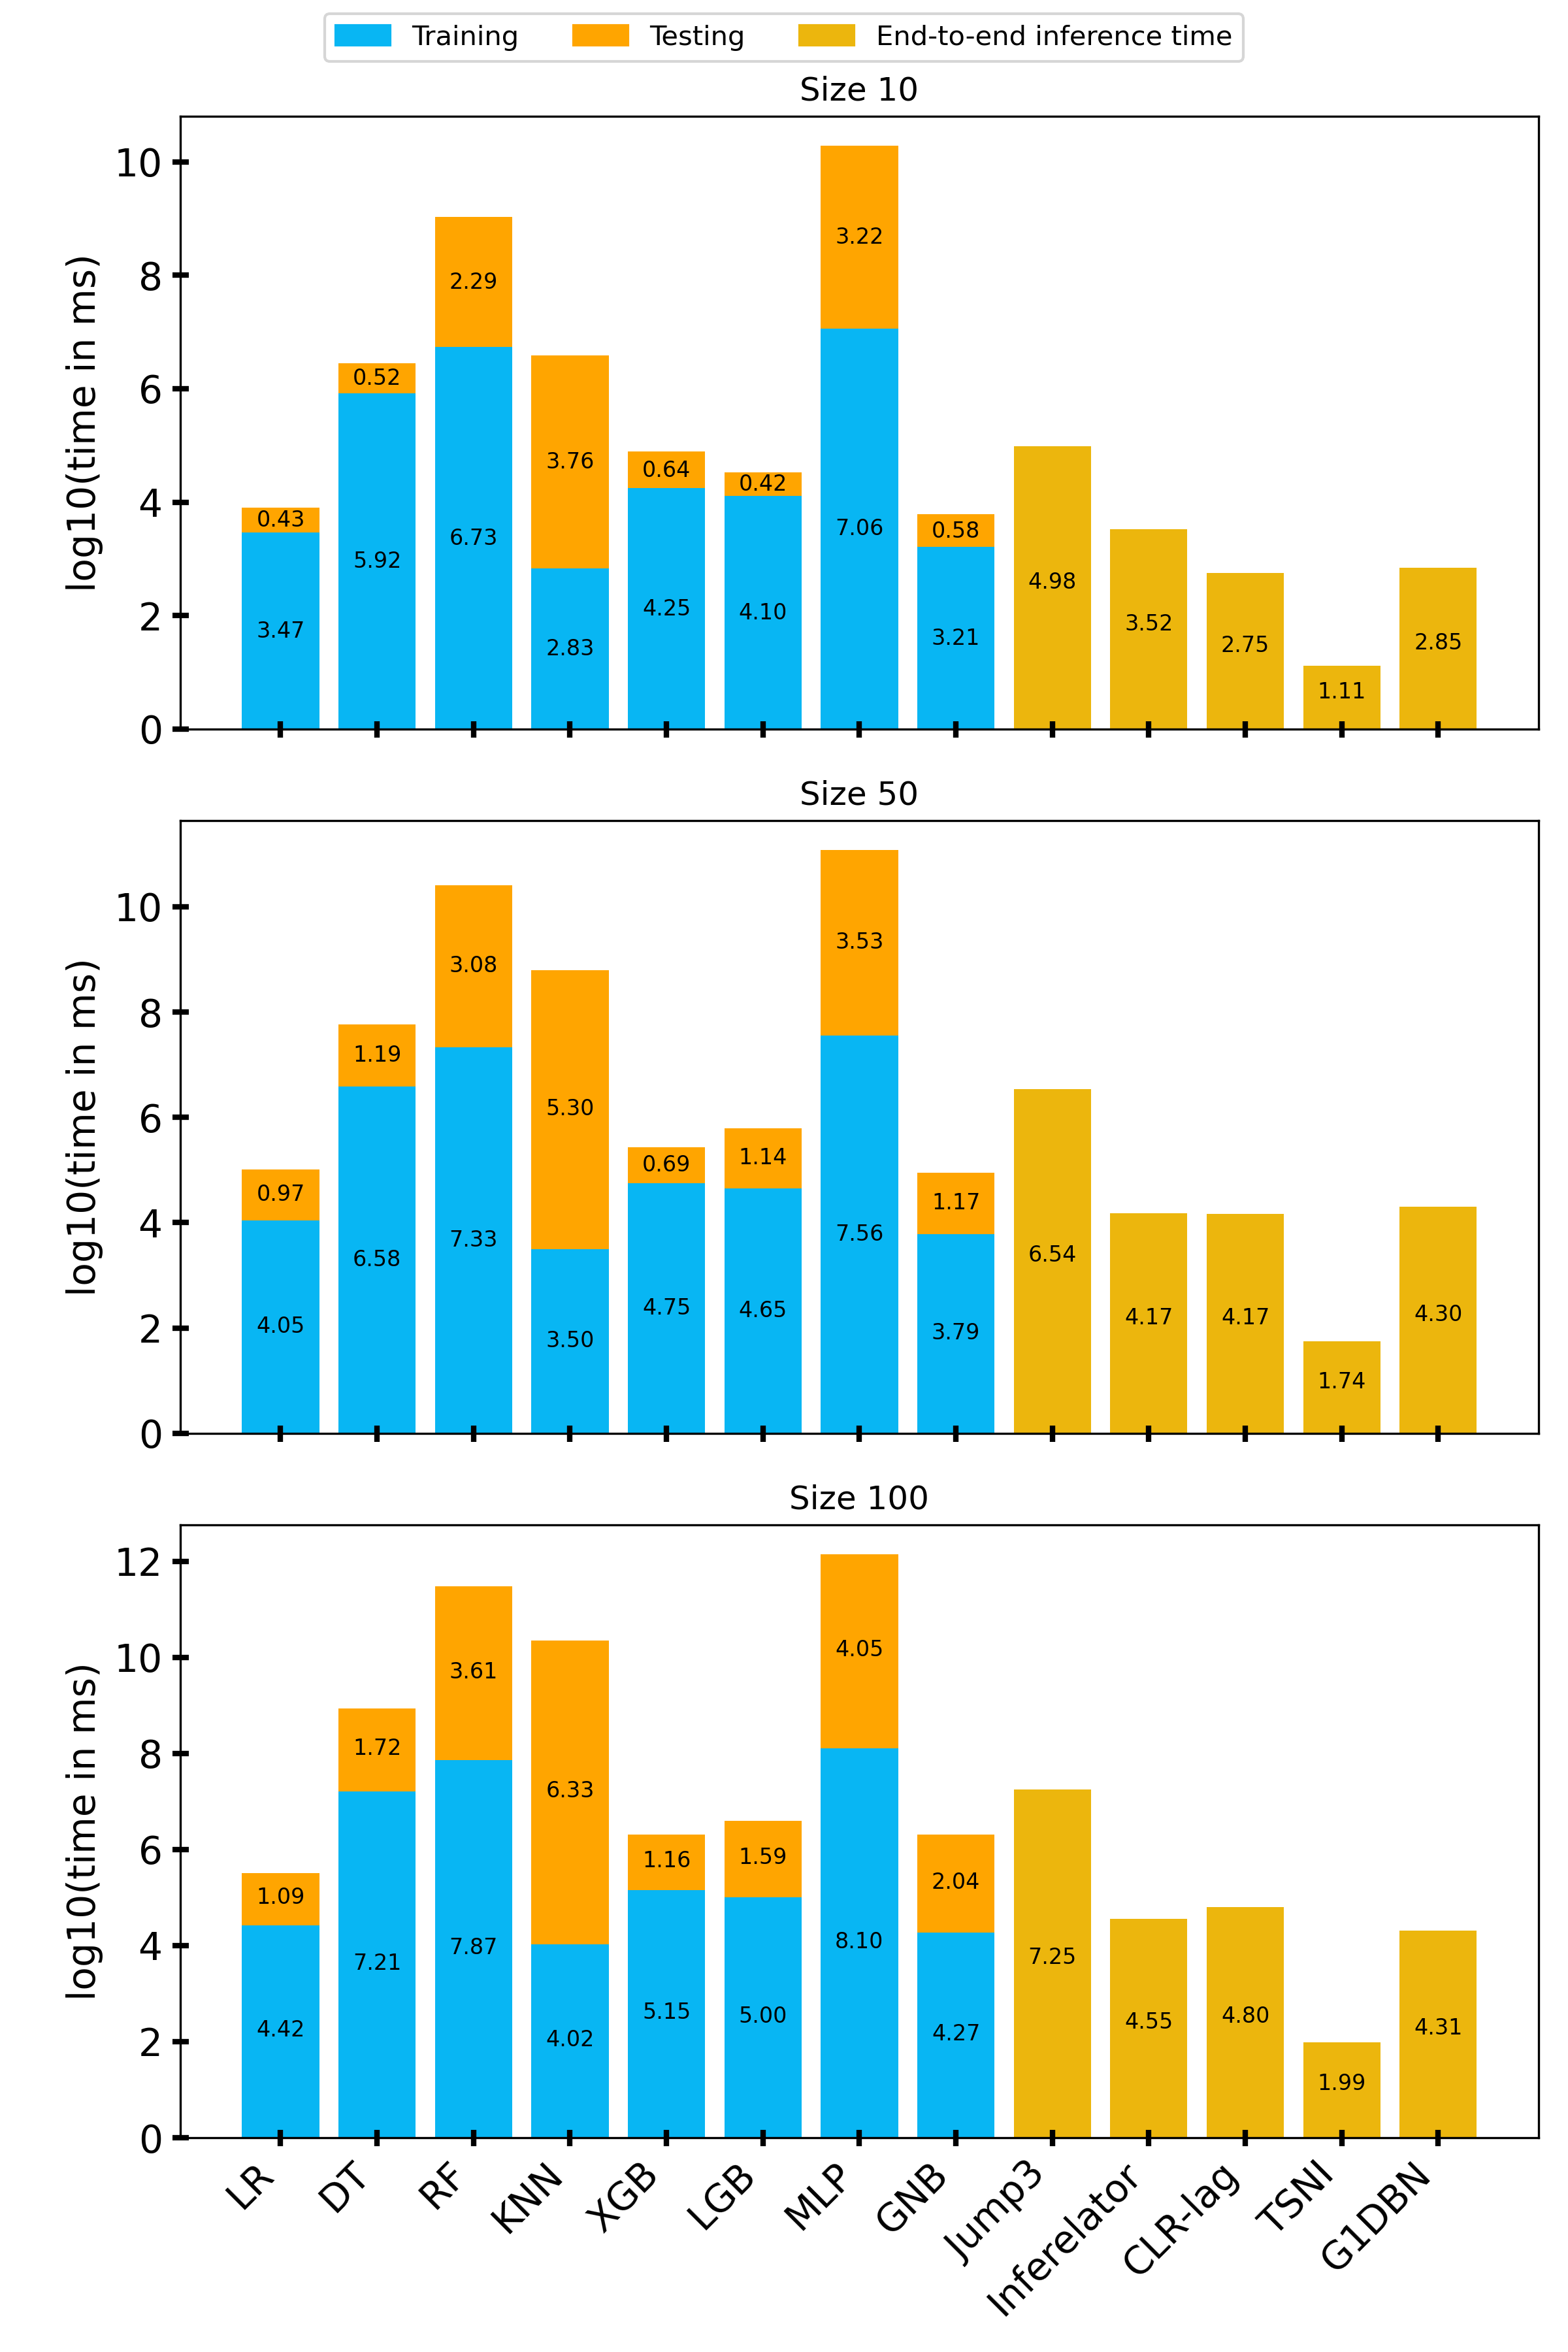
\includegraphics[width=1.0\linewidth]{Figures/chapter3_running_time.png}
\caption{Comparison of running time across different GRN inference methods on the \textit{E. coli} dataset for network sizes 10, 50, and 100. The y-axis shows the logarithm base 10 of the running time measured in milliseconds, while the x-axis represents the evaluated inference methods. Results highlight the trade off between higher initial training cost and faster inference for learning-based methods, particularly in scenarios involving repeated network inference.}\label{chapter3_running_time_figure}
\end{figure}

\subsection{Running time}
We further evaluated the computational efficiency of the proposed framework by analyzing its running time in comparison with representative baseline methods. The experiments were conducted on a workstation equipped with an Intel(R) Xeon Silver 4210R CPU at 2.40 GHz, \texttt{x86\_64} architecture, and 64 GB RAM. All reported values correspond to the logarithm base 10 of the running time measured in milliseconds.

The comparison was performed on three \textit{E. coli} network sizes, namely 10, 50, and 100 genes. For learning-based methods, the running time was decomposed into two components: training time and inference (testing) time. In contrast, methods such as Jump3, Inferelator, CLR-lag, TSNI, and G1DBN do not involve an explicit training phase; therefore, their reported running time corresponds to the end-to-end inference time, measured from the start of execution until the inferred network is obtained. Details of the datasets used for training and testing are provided in Table ~\ref{chapter3_ecoli_dataset}.

As shown in the Figure ~\ref{chapter3_running_time_figure}, the running time comparison across all three network sizes, the training time of learning-based methods is generally higher than the inference time of direct GRN inference algorithms such as Jump3 and CLR-lag. This behavior is expected, as the former require an explicit model learning phase, whereas the latter directly infer the network structure from the input data without prior training. However, once trained, the learning-based methods exhibit substantially lower inference time compared to the end-to-end inference time of the direct methods.

This distinction becomes particularly important in scenarios where a large number of networks need to be inferred. For the proposed framework and other learning-based approaches, the training process is performed only once, after which the trained model can be reused to infer multiple networks efficiently. Consequently, the overall computational cost scales primarily with the inference time, which remains relatively small. In contrast, direct inference methods incur a similar computational cost for each network, as the entire inference procedure must be executed independently for every instance. As a result, their total running time increases linearly with the number of networks, making them less efficient when applied to large-scale or repeated inference tasks.


\section{Discussion and Conclusion}
The proposed framework demonstrates stable performance across both discrete and continuous datasets, highlighting robustness under diverse data generation regimes in gene regulatory network inference. By introducing an interaction level representation that jointly encodes temporal expression dynamics and regulatory structure, the framework enables the effective use of a broad range of machine learning classifiers and consistently outperforms traditional approaches based solely on temporal profiles. A key advantage of the framework is its assumption free design. In contrast to many existing methods that rely on heuristic choices such as predefined time lags or fixed candidate regulator sets, the proposed representation avoids explicit parametric assumptions about regulatory dynamics. This improves robustness across datasets and reduces the need for extensive parameter tuning. From a practical standpoint, the framework provides a well-defined inference protocol for unseen data. Inference is feasible when the temporal length of new expression profiles matches or exceeds that used during training through temporal alignment. When time series are shorter, direct inference is not possible and temporal extension techniques are required \parencite{anh2025}, explicitly defining the current scope and limitation of the method. Importantly, the proposed representation is scale invariant, as regulatory interactions are encoded independently of global network size. This property enables effective generalization across networks of different sizes and allows training data to be augmented with interaction samples from heterogeneous network scales, mitigating class imbalance. Together, by addressing shared limitations of existing task transformation approaches, including fragile assumptions, limited scalability, and weak cross network generalization, the proposed framework provides a flexible and scalable foundation for time series GRN inference and supports robust deployment in practical biological settings.